\documentclass{article}
\usepackage[utf8]{inputenc}
\usepackage[margin=2.5cm]{geometry}

\usepackage{graphicx}
\usepackage{color}
\usepackage{xspace}
\newcommand{\seb}[1]{\xspace\textcolor{red}{#1}\xspace}

% maths
\usepackage{amsmath}
\usepackage{amssymb}
\usepackage{amsthm}
\newcommand{\PR}{\mathbb{P}}

% bibliography
\usepackage[round, sort&compress]{natbib}
\usepackage{har2nat}
\bibliographystyle{agsm}

% custom header/footer
\usepackage{fancyhdr}
\pagestyle{fancy}
\renewcommand{\headrulewidth}{0pt}
\fancyhf{}
\rfoot{\textsf{\thepage}}
\lfoot{\textsf{Suzie Brown}}

\title{Ancestor Sampling}
\author{Suzie Brown}
\date{\today}

\begin{document}
\maketitle
\thispagestyle{fancy}

Ancestor sampling was first suggested by Nick Whiteley in the discussion on \citet{andrieu2010}. Its contribution is to reduce autocorrelation between samples obtained using the particle Gibbs algorithm \citep{andrieu2010}.
\seb{Proper way to cite discussion of paper?}


\section*{The particle Gibbs algorithm}

The scenario we present is a particle Gibbs algorithm for filtering with unknown parameters. The method applies more generally to particle Gibbs (for which the reader is directed to \citet[Chapter 5]{lindsten2013}), but we find this particular scenario to be simple and instructive. \seb{To generalise to Del Moral's SMC framework basically requires just the change of notation $g \to G_t, f \to M_t$.}

Consider the following hidden Markov model, parametrised by a constant parameter $\theta$ which may be multidimensional.
\seb{Define the spaces in which theta,X,Y live?}
\begin{align*}
Y_t \mid X_t &\sim g_\theta(\cdot \mid X_t)\\
X_{t} \mid X_{t-1} &\sim f_\theta(\cdot \mid X_{t-1})\\
X_0 &\sim \mu_\theta(\cdot) \\
\theta &\sim p(\cdot)
\end{align*}
\seb{Add ranges for t in first two lines.}
\seb{Use q instead of f for better congruity with other sections?}
We work on a fixed time horizon $T \in \mathbb{N}$, which is necessary to implement the particle Gibbs algorithm.
\seb{Can be artifically imposed by block sampling if doing online-ish inference?}
The measures corresponding to $\mu_\theta$, $f_\theta$ and $g_\theta$ are assumed to be known and to admit densities, and we are also given a fixed sequence of observations $y_{1:T}$. 
\seb{Either mention that f,g can depend on t, or make this explicit  in the notation.}
\seb{Don't really need to include prior on theta; it's not relevant to CSMC step.}

Our aim is to generate Monte Carlo samples from the joint distribution of $X_{0:T}$ and $\theta$ conditional on $y_{1:T}$. Outside of models admitting closed-form solutions, this is typically the most practical way to draw samples from the marginal distributions of either $theta$ or any subset of the states $X_{0:T}$, by marginalising the Monte Carlo samples. 

The structure of the model invites Gibbs sampling: alternating between updating $\theta$ conditional on $X_{0:T}$, and updating $X_{0:T}$ conditional on $\theta$.
\seb{``These conditionals are typically much easier to sample from that the corresponding marginals.'' (due to the dependence structure in the HMM).}
The $\theta$ update consists of sampling from 
\begin{equation*}
p(\theta \mid x_{0:T}, y_{1:T}) \propto p(\theta) p(x_{0:T}, y_{1:T} \mid \theta) ,
\end{equation*}
which can be achieved quite easily with a Metropolis--Hastings step.
The $X$ update is the `difficult' part, requiring a sample from
\begin{equation*}
p(x_{0:T} \mid \theta , y_{1:T}) =: \gamma_T^\theta(x_{0:T}) .
\end{equation*}
\seb{Define gamma for general s too:
\begin{equation*}
\gamma_s^\theta(x_{0:s}) \propto \mu_\theta(x_0) g_\theta(y_0\mid x_0) \prod_{r=1}^s f_\theta(x_r \mid x_{r-1}) g_\theta(y_r \mid x_r) .
\end{equation*}
}
This target distribution is suited to sequential Monte Carlo, and this is where the `particle' part of particle Gibbs comes in.
We update all of the hidden states $X_{0:T}$ in one Gibbs step, which consists of drawing one sample from a particle filter. To target the correct distribution, we use conditional SMC for these updates, conditional on the sample of $X_{0:T}$ from the previous sweep. 

[Refer back to the CSMC algorithm which I've already written down somewhere, explaining how the inputs to the algorithm correspond to functions/quantities introduced in this setting.]


\section*{Ancestral degeneracy leads to poor mixing}

Particle Gibbs runs into problems when the time horizon $T$ is large compared to the number of particles $N$. $T$ is determined by the application at hand, and $N$ is limited by computational resources, so we may not be able to control their relative size. 
The source of the problem is ancestral degeneracy. 
We know that in standard SMC algorithms this problem exists and its effect is to increase the variance of our Monte Carlo estimates. 
In particle Gibbs, the $N$ simulated trajectories are not used to estimate anything; only one trajectory is sampled at each step, and becomes one state a Markov chain Monte Carlo estimate. Ancestral degeneracy now has a less direct effect: it causes the Markov chain to mix slowly. 

\begin{figure}
\centering
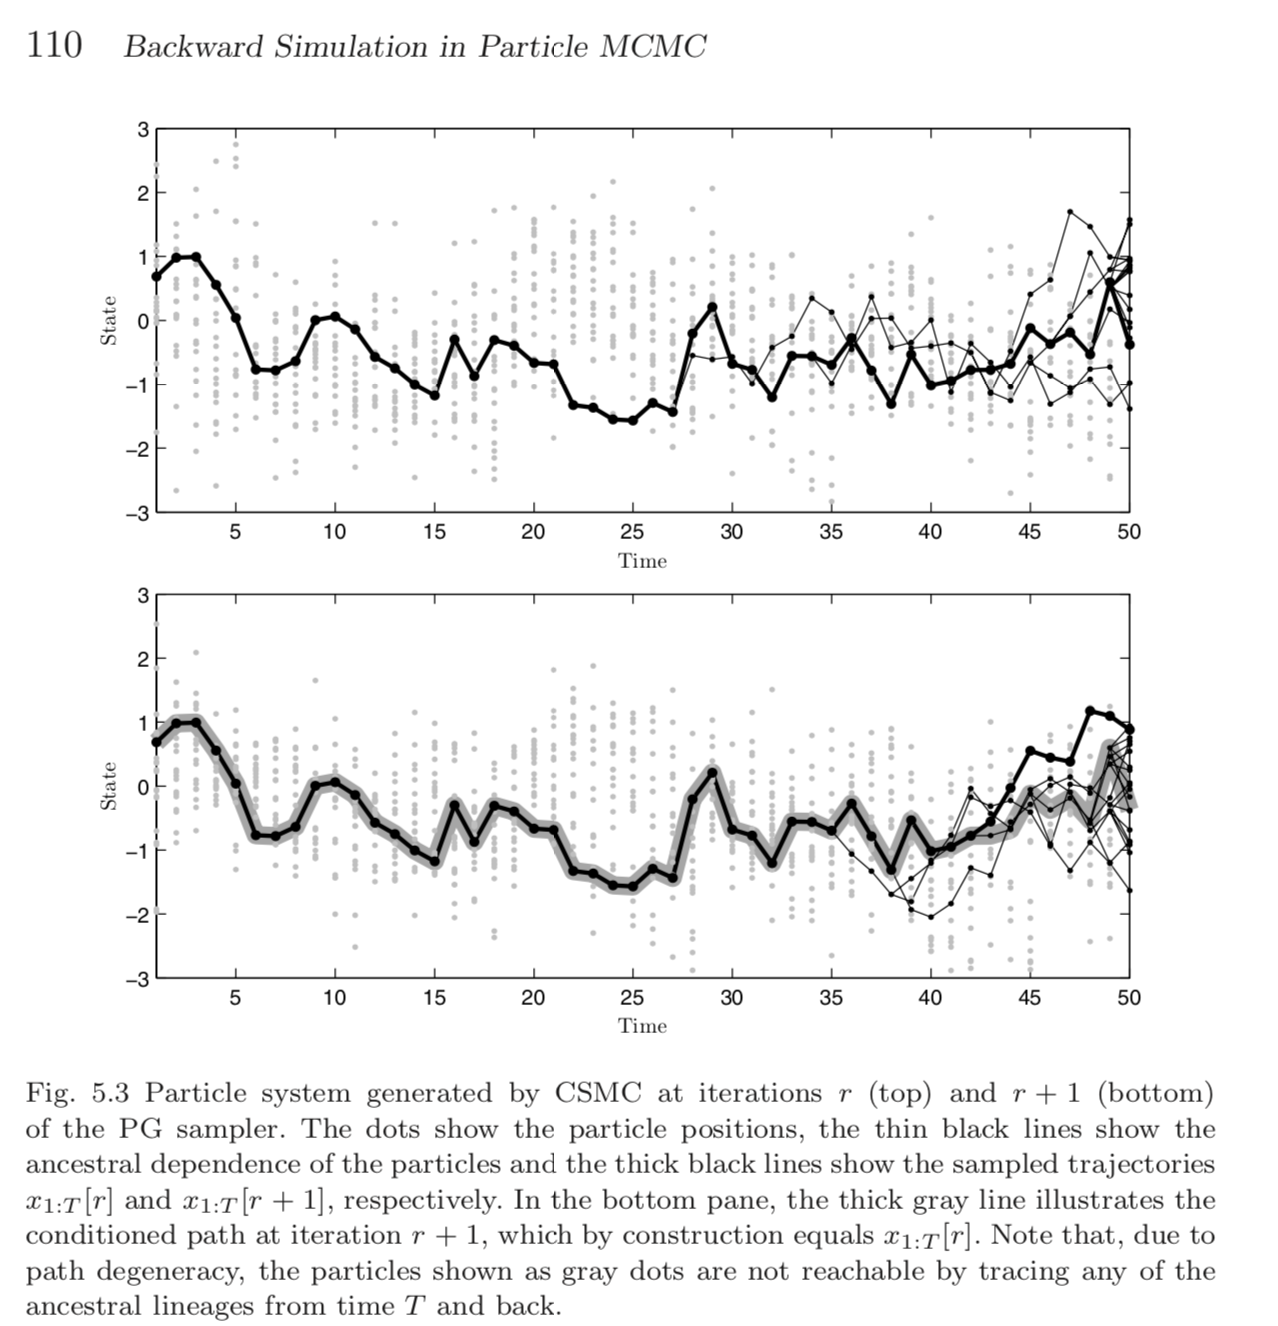
\includegraphics[width=0.8\textwidth]{lindsten_figure.png}
\caption{A placeholder copied from \citet{lindsten2013}.}
\label{fig:PG_ancdegen}
\end{figure}

To see why, take a look at Figure \ref{fig:PG_ancdegen}. In Figure \ref{fig:PG_ancdegen}a we have just completed the $r^{th}$ Gibbs sweep, sampling $\theta[r]$ and $x_{0:T}[r]$. For the $(r+1)^{th}$ sweep, we take as immortal trajectory $x_{0:T}^* = x_{0:T}[r]$, and run conditional SMC. Due to ancestral degeneracy, many of the resulting trajectories coalesce, and since the immortal trajectory must survive across the whole time window, they tend to coalesce onto the immortal trajectory (Figure \ref{fig:PG_ancdegen}b). Now we obtain the next sample $x_{0:T}[r+1]$ by sampling a trajectory among the $N$ we have just simulated. Whichever one we choose, it has a high amount of overlap with the immortal trajectory, i.e.\ the previous sample $x_{0:T}[r]$. This behaviour tends to repeat at every iteration, meaning the early $X$ coordinates are getting `stuck' (rarely being updated). This is clearly a problem for the mixing of the Markov chain.
\seb{Another way to explain this is that the variables defining the immortal trajectory (indices and states) are never refreshed during the Gibbs sweep - this is the explanation given in Lindsten Ch5.}
It renders the particle Gibbs algorithm impractical for any such model where the time horizon $T$ is too large: either we must run the Markov chain for longer, or increase the number of particles $N$ in the conditional SMC step, neither of which is feasible on a limited computational budget. 


\section*{The solution: ancestor sampling}

An effective solution (where it is possible to implement it) was proposed by Nick Whiteley and is known as ancestor sampling.
It consists of a simple modification to the resampling step within the conditional SMC algorithm. 
In the basic CSMC algorithm, at each time step the particles are resampled by multinomial resampling according to their weights. That is, at each time $t$, each non-immortal offspring is assigned a parent as so:
\begin{equation*}
\PR[a_t^{(j)} = i] \propto w_t^{(i)} ,
\end{equation*}
while the immortal offspring is deterministically assigned to the immortal parent.

\begin{figure}
\centering
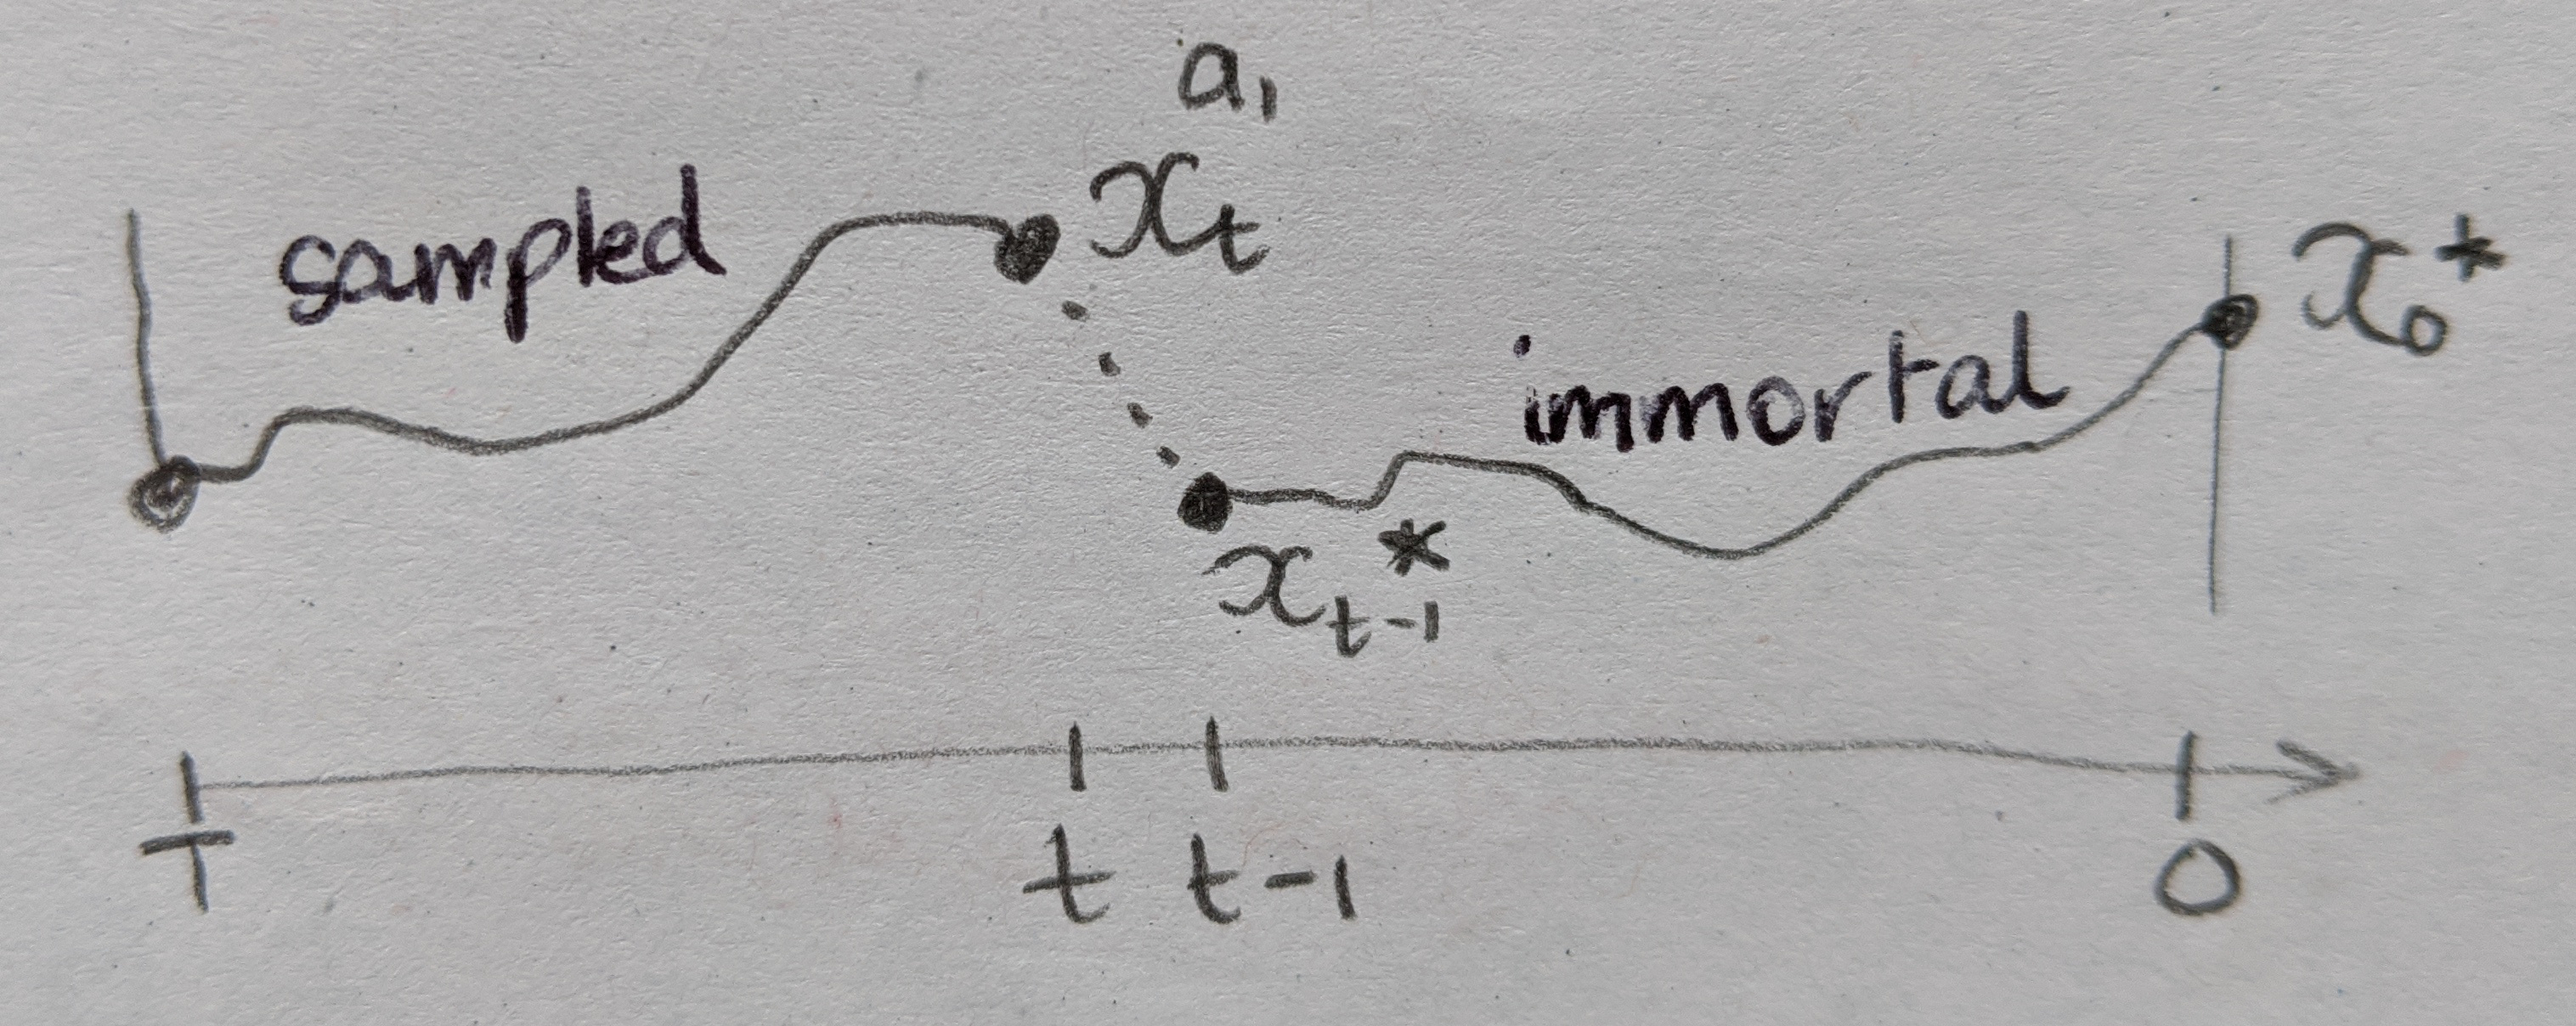
\includegraphics[width=0.8\textwidth]{immresample.jpg}
\caption{Interpretation of a resampling weight for the immortal offspring.}
\label{fig:resample_immortal}
\end{figure}

In ancestor sampling we do the same thing, except that the immortal particle is also resampled, rather than being deterministically assigned:
\begin{equation*}
\PR[a_t^{(j)} = i] \propto
\begin{cases}
w_t^{(i)} &\text{non-immortal particles}\\
w_t^{(i)} \frac{\gamma_T^\theta((x_{0:t-1}^{(i)}, x_{t:T}^*))}{\gamma_{t-1}^\theta(x_{0:t-1}^{(i)})} &\text{immortal particle} .
\end{cases}
\end{equation*}
The ratio of $\gamma$s can be interpreted as the conditional probability of the trajectory continuing with $x_{t:T}^*$ given is starts with $x_{0:t-1}^{(i)}$ (see Figure \ref{fig:resample_immortal}).
Using the structure of the hidden Markov model defined earlier, we can rewrite the ratio
\begin{equation*}
\frac{\gamma_T^\theta((x_{0:t-1}^{(i)}, x_{t:T}^*))}{\gamma_{t-1}^\theta(x_{0:t-1}^{(i)})}
\propto f_\theta(x_t^* \mid x_{t-1}^{(i)}) g_\theta(y_t \mid x_t^*) \prod_{s=t}^T f_\theta(x_r^* \mid x_{r-1}^*) g_\theta(y_r \mid x_r^*)
\propto f_\theta(x_t^* \mid x_{t-1}^{(i)}) .
\end{equation*}
\seb{Should the first propto actually be equality?}
So it looks like it should also be pretty easy to implement ancestor sampling for our model. \seb{Write down the pseudocode to prove it?}
The only catch is that we need to be able to evaluate $f_\theta$ pointwise, whereas in the basic algorithm we only need to draw samples from $f_\theta$. This will rule out ancestor sampling in some applications.


\section*{Why ancestor sampling works}

Ancestor sampling is backward sampling, but only for the immortal trajectory. (It isn't possible to do backward sampling during the forward sweep for any except the immortal trajectory - see that we can't evaluate the required $\gamma$s without knowing the future states, which are known only for the immortal trajectory.)
We know that backward sampling (on all trajectories, in a separate backward sweep) eradicates ancestral degeneracy. But we've only backward-sampled one trajectory, leaving the other $N-1$ trajectories to do their coalescing thing.

The important point is that ancestor sampling does not prevent ancestral degeneracy (it mitigates it a tiny bit like $1/N$). Ancestral degeneracy is pretty much as severe as ever; the difference is that the trajectories no longer coalesce preferentially onto the immortal trajectory. There is no longer an immortal trajectory to coalesce onto. An illustration of this can be seen in Figure \ref{fig:whyASworks}.

\begin{figure}
\centering
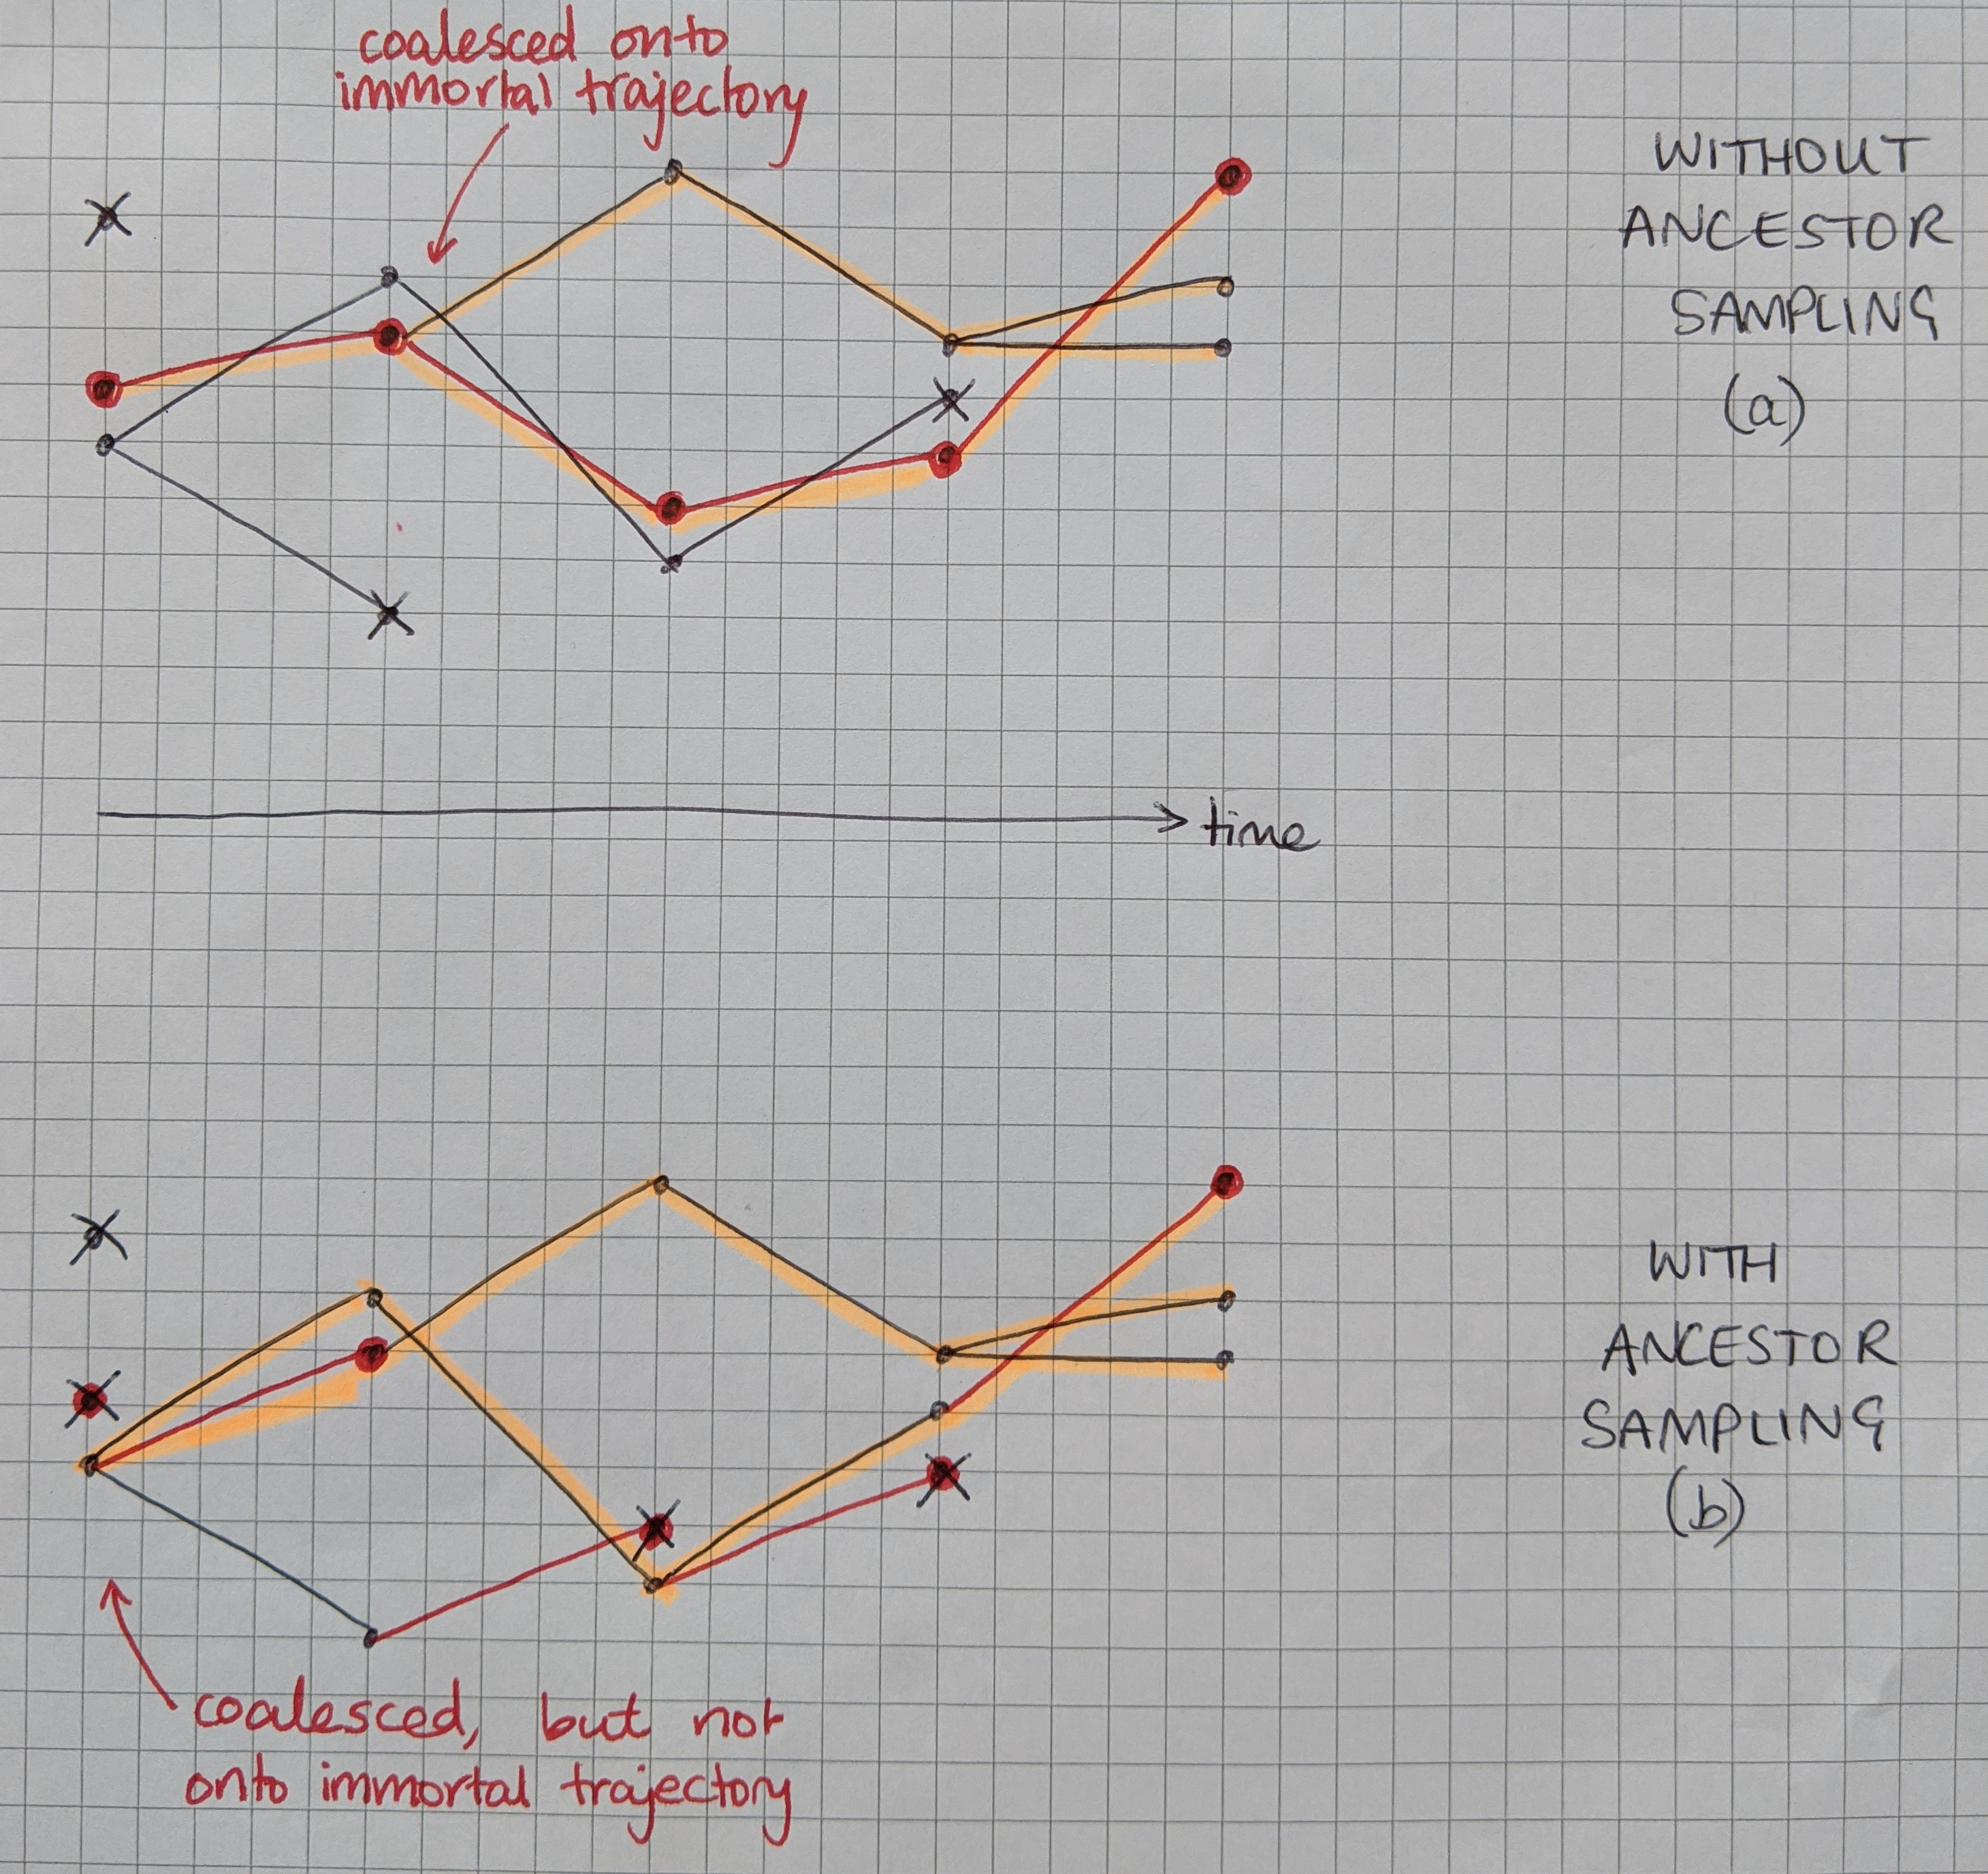
\includegraphics[width=0.8\textwidth]{ancsampworks.jpg}
\caption{Illustration of how ancestor sampling prevents coalescence onto the immortal trajectory.}
\label{fig:whyASworks}
\end{figure}

Remember, the problem with ancestral degeneracy in particle Gibbs was that it induced strong autocorrelation among consecutive samples of $X_{0:T}$. It isn't a problem that the trajectories coalesce, as long as the thing they coalesce to is able to move, readily exploring the state space. This is achieved with ancestor sampling.

\seb{Why is ancestor sampling even a valid thing to do (i.e. still targetting the right thing)? Extended state space argument?(I think there is one in Lindsten Ch5). No need to go into it here unless there is a simple intuitive explanation to put the reader's mind at rest.}


\section*{The genealogical perspective}

Ancestor sampling interrupts the immortal trajectory, splitting it into disjoint pieces (see Figure \ref{fig:whyASworks}b). So perhaps it doesn't make sense to talk about genealogies, now that we don't have a strictly coalescing process evolving backwards in time.

\seb{Probably need some conditioning e.g.\ on $\mathcal{H}_t$ in the following equations.}
But let's look at this resampling scheme backwards in time anyway. With the time indices now reversed, and the notation made consistent with our work on genealogies, we have
\begin{equation*}
\PR[a_t^{(j)} = a_i] \propto
\begin{cases}
w_t^{(a_i)} q_{t-1}(X_t^{(a_i)}, X_{t-1}^{(j)}) &\text{non-immortal particles}\\
w_t^{(a_i)} q_{t-1}(X_t^{(a_i)}, X_{t-1}^*) &\text{immortal particle} .
\end{cases} .
\end{equation*}
\seb{Might be neater to avoid bringing in $j$ at all, and write $a_t^{(i)} = a_i$ etc.}
But when $j$ is the index of the immortal particle, $X_{t-1}^{(j)} = X_{t-1}^*$, so the reverse-time view makes no distinction between the immortal particle and others in terms of how their parents are chosen. We have
\begin{equation*}
\PR[a_t^{(j)} = a_i] \propto
w_t^{(a_i)} q_{t-1}(X_t^{(a_i)}, X_{t-1}^{(j)})
\end{equation*}
for all particles. 
This is the same probability we get with multinomial resampling in standard SMC.

This viewpoint gives us another intuition about the effect of ancestor sampling: the immortal particle is no longer specially favoured when it comes to producing offspring. In the basic algorithm, the immortal parent produces on average one more offspring at each generation than any other parent (and must produce at least one offspring). It follows that the immortal line cannot die out (is immortal), and also that it is a more likely site for coalescence events (i.e.\ producing at least two offspring) than any other parent. 
With ancestor sampling, the immortal parent loses this advantage; it is treated just like the other parents. It is no longer a particularly favourable site for coalescing, so the trajectory onto which everyone coalesces might just as well be any of the other $N-1$ trajectories. This prevents the Markov chain getting stuck as in Figure \ref{fig:PG_ancdegen}.


\bibliography{../smc.bib}
\end{document}